\documentclass[10pt,a4paper]{article}

% Português
\usepackage[utf8]{inputenc}
\usepackage[T1]{fontenc}
\usepackage[portuguese]{babel}

% Fonte Arial (Helvetica)
\usepackage{helvet}
\renewcommand{\familydefault}{\sfdefault}

% Layout e formatação
\usepackage[margin=2cm,top=1.5cm,bottom=2cm]{geometry}
\usepackage{multicol}
\usepackage{xcolor}
\usepackage{tikz}
\usetikzlibrary{positioning}
\usepackage{titlesec}
\usepackage{lettrine}
\usepackage{setspace}

% Matemática e símbolos
\usepackage{amsmath}
\usepackage{amsfonts}
\usepackage{amssymb}

% Figuras e tabelas
\usepackage{graphicx}
\usepackage{float}
\usepackage{booktabs}
\usepackage{array}
\usepackage{caption}

% Configuração de captions
\captionsetup[figure]{labelfont=bf}

% Códigos
\usepackage{listings}
\usepackage{xcolor}

% Configuração do listings
\lstset{
    basicstyle=\ttfamily\footnotesize,
    numbers=left,
    numberstyle=\tiny\color{gray},
    stepnumber=1,
    numbersep=5pt,
    backgroundcolor=\color{gray!10},
    showspaces=false,
    showstringspaces=false,
    showtabs=false,
    frame=single,
    rulecolor=\color{black},
    tabsize=2,
    captionpos=b,
    breaklines=true,
    breakatwhitespace=false,
    language=Python
}

% Citações e referências
\usepackage[style=abnt,backend=biber]{biblatex}
\addbibresource{referencias.bib}

% Links
\usepackage[colorlinks=false,pdfborder={0 0 0}]{hyperref}

% Definir cores personalizadas
\definecolor{cyanline}{RGB}{0,174,239}
\definecolor{linkcolor}{RGB}{0,174,239}

% Tipografia
\setlength{\parindent}{0pt}
\setlength{\parskip}{6pt}
\setlength{\columnsep}{20pt}

% Títulos
\titleformat{\section}
{\normalfont\large\bfseries}
{\thesection}{1em}{}

% Configuração do cabeçalho
\usepackage{fancyhdr}
\pagestyle{empty}

% Linha Azul
\newcommand{\thinline}{%
    \noindent\textcolor{cyanline}{\rule{\textwidth}{1pt}}
}

% Comando para o cabeçalho
\newcommand{\makeheader}[5]{%
    \thinline
    \vspace{0.05cm}
    
    {\Huge\bfseries #1}
    \vspace{0.5cm}

    \begin{minipage}[t]{0.7\textwidth}
        {\footnotesize $^1$#2}\\[0.3cm]
    \end{minipage}
    \hfill
    \begin{minipage}[t]{0.28\textwidth}
        \raggedleft
        \footnotesize
        #3\\
        #4
    \end{minipage}
    \vspace{0.05cm}
    \thinline
    \vspace{0.2cm}
}

% Comando para data
\newcommand{\makedate}[1]{%
    \begin{center}
        \large #1
    \end{center}
    \vspace{0.05cm}
}

\begin{document}

% Cabeçalho
\makeheader{Análise epidemiológica de HIV/AIDS no estado da Paraíba}{Bacharelado em Ciência da Computação}{Estudo de Visualização de Dados}{Centro de Informática - UFPB}

% Data
\makedate{09 de setembro de 2025}

% Início das duas colunas
\begin{multicols}{2}

    \lettrine[lines=2]{\textcolor{cyanline}{E}}{} {\bfseries ste trabalho tem como objetivo principal apresentar, de forma sucinta e informativa, uma análise exploratória dos casos de HIV/AIDS no estado da Paraíba durante o período de 2019 a 2024, utilizando dados provenientes do IBGE e do sistema DataSUS. Propõe-se uma análise que forneça explicabilidade aos dados, dessa forma, buscamos fornecer insights relevantes que possam auxiliar o poder público na formulação e direcionamento de ações preventivas, especialmente no contexto pós-introdução do medicamento lenacapavir, contribuindo para o bom aproveitamento de recursos públicos.}

\section{Escopo}

Este projeto insere-se no campo científico da \textbf{Epidemiologia}, especificamente na área de epidemiologia descritiva de doenças infecciosas, com interface direta com as disciplinas de \textbf{Saúde Pública} e \textbf{Ciência da Computação}. O domínio de expertise abrange a aplicação de métodos epidemiológicos para análise de dados secundários em saúde, visando uma compreensão abrangente do impacto do HIV/AIDS na sociedade e contribuindo para o desenvolvimento de estratégias mais eficazes de prevenção, tratamento e controle da doença.

A análise epidemiológica dos casos de HIV/AIDS no estado da Paraíba constitui-se como ferramenta fundamental para identificar padrões de distribuição geográfica e demográfica, caracterizar o perfil das populações mais vulneráveis e fornecer informações essenciais para a formulação de políticas públicas direcionadas. Esta abordagem metodológica permite subsidiar ações mais efetivas e otimizar a alocação de recursos públicos limitados.

O escopo metodológico compreende a análise exploratória de dados (EDA), visualização científica de informações epidemiológicas e aplicação de princípios de epidemiologia descritiva segundo as dimensões clássicas de pessoa, lugar e tempo.

A relevância deste trabalho é reforçada pelo contexto atual das políticas de prevenção ao HIV. Em julho de 2025, a Organização Mundial da Saúde (OMS) publicou diretrizes oficiais recomendando o uso do lenacapavir injetável como uma nova estratégia de prevenção do HIV, destacando seu potencial para ampliar o acesso e a efetividade das ações preventivas, especialmente em populações mais vulneráveis~\cite{oms_lenacapavir_2025}. Essa recomendação internacional evidencia a necessidade de análises epidemiológicas regionais, como a proposta neste estudo, para subsidiar a implementação e o monitoramento de novas intervenções no contexto local.

\section{Desafio}

Do ponto de vista tecnológico, o desafio reside na integração e harmonização de múltiplas bases de dados heterogêneas (DATASUS, IBGE), que apresentam diferentes estruturas, periodicidades e níveis de granularidade. A transformação desses dados brutos em informações epidemiológicas interpretáveis e acionáveis requer o desenvolvimento de pipelines analíticos robustos e técnicas avançadas de visualização que comuniquem efetivamente padrões complexos para diferentes audiências.

O desafio operacional central é a tradução dos achados epidemiológicos em recomendações práticas para gestores de saúde pública, considerando as limitações orçamentárias e logísticas do Sistema Único de Saúde (SUS) no contexto estadual.

Adicionalmente, existe o desafio de comunicação científica: como apresentar análises epidemiológicas complexas de forma acessível e convincente para gestores públicos, profissionais de saúde e sociedade civil, garantindo que os insights gerados sejam efetivamente incorporados ao processo decisório em saúde pública.

\section{Projeto de visualização}

O projeto de visualização segue um modelo estruturado e envolve as seguintes etapas:

\textbf{1. Entrada:} foram coletadas múltiplas bases de dados epidemiológicos e demográficos, constituindo o objeto de estudo e de geração das representações visuais (RVs). Os dados epidemiológicos sobre HIV/AIDS foram extraídos do sistema DATASUS~\cite{datasus_tabnet}, abrangendo quatro bases distintas: casos por município, distribuição por sexo, faixa etária e valores de internação. Os dados demográficos da Paraíba foram obtidos do IBGE~\cite{ibge_paraiba}, incluindo informações populacionais do censo 2022, além da malha territorial através de shapefile~\cite{ibge_malhas}. Todas as bases foram importadas através da biblioteca pandas.

\textbf{2. Pré-Processamento:} foram realizadas transformações essenciais para limpeza e harmonização dos dados, incluindo padronização de nomes de municípios, tratamento de valores ausentes e cálculo da taxa de incidência por 100.000 habitantes.

\textbf{3. Mapeamento:} foi estabelecido um projeto gráfico baseado em questionamentos epidemiológicos fundamentais, definindo paleta de cores e estruturas visuais adequadas para representar distribuições geográficas, temporais e demográficas dos casos de HIV/AIDS.

\textbf{4. Visualização:} etapa final que apresenta as RVs através de mapas da distribuição de casos por município, análises temporais da evolução epidemiológica e caracterização demográfica por sexo e faixa etária, subsidiando a tomada de decisão em saúde pública.

\section{Mapeamento}

O tratamento dos dados (codificação resumida) foi realizado sobre as bases de dados epidemiológicos do DATASUS e demográficos do IBGE, que por sua vez foram processadas através de técnicas de ETL (Extrair, Transformar e Carregar) utilizando Python.

\textbf{Processamento das Bases DATASUS}

Os códigos abaixo sintetizam o tratamento realizado para limpeza e união das quatro bases epidemiológicas em dataframes estruturados:

\begin{lstlisting}
import pandas as pd

# Importacao das bases DATASUS e IBGE
df_mun = pd.read_csv('datasus_hiv_mun_2019-2024.csv', sep=';')
df_sex = pd.read_csv('datasus_hiv_sex_data_2019-2024.csv', sep=';')
df_sex_age = pd.read_csv('datasus_hiv_sex_idade_2019-2024.csv', sep=';')
df_mun_val = pd.read_csv('datasus_hiv_mun_valor_2019-2024.csv', sep=';')
df_pop = pd.read_excel("ibge_pb_mun.xlsx")

# Limpeza e padronizacao
df_mun['Municipio'] = df_mun['Municipio'].astype(str).str.replace(r'^\d+\s+', '', regex=True)
df_mun_val['Municipio'] = df_mun_val['Municipio'].astype(str).str.replace(r'^\d+\s+', '', regex=True)
\end{lstlisting}

\textbf{União com Dados Demográficos}

O IBGE forneceu informações populacionais que, após união com os dados epidemiológicos (código abaixo), produziram o dataframe para cálculo de taxas de incidência:

\begin{lstlisting}
# Padronizacao para merge
df_pop['Municipio'] = df_pop['Municipio'].apply(
    lambda x: remove_accents(str(x)).upper())

# Uniao das bases
df_final = df_mun_2022.merge(df_pop, on='Municipio')
df_final['Taxa_100mil'] = (df_final['Casos'] / 
                           df_final['Populacao']) * 100000

# Filtro para municipios com populacao >= 10.000 hab
df_final = df_final[df_final['Populacao'] >= 10000]
\end{lstlisting}

A Figura 1 apresenta o resultado do processo de união das bases epidemiológicas com os dados populacionais, exemplificando a estrutura final dos dados após o tratamento, incluindo os municípios paraibanos com suas respectivas distribuições mensais de casos, população e taxa calculada por 100.000 habitantes.

\begin{figure}[H]
    \centering
    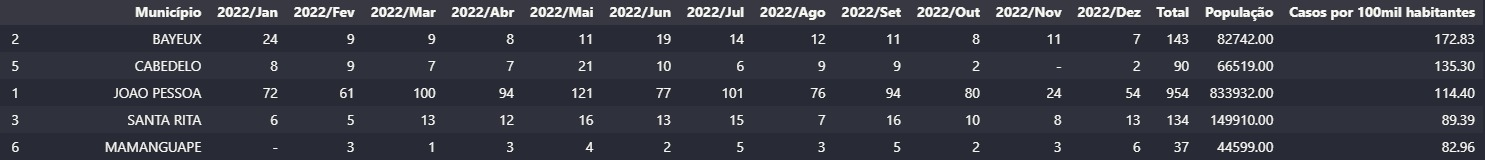
\includegraphics[width=\linewidth]{merged_dataset.jpeg}
    \caption{\textit{Dataframe} pós merge}
    \label{fig:dataframe_merge}
\end{figure}

Destaca-se que na construção da análise de taxa por 100.000 habitantes foram desconsiderados os casos de municípios com menos de 10.000 habitantes, visto que a baixa população poderia gerar inconsistências na análise, resultando em taxas artificialmente elevadas que não representariam adequadamente o cenário epidemiológico real.

No mais, os dados geoespaciais foram adquiridos através do shapefile do IBGE, permitindo a criação de mapas coropléticos para visualização da distribuição geográfica dos casos de HIV/AIDS no estado da Paraíba.

\section{Representações Visuais}

As RVs estão dispostas a seguir, seguindo todo o processo mencionado no projeto de visualização .

\textbf{Evolução Temporal dos Casos}

A Figura 2 representa a progressão anual dos casos de HIV/AIDS na Paraíba. Do ponto de vista visual, pode-se notar que as barras possuem coloração uniforme em tom azul, facilitando a comparação direta entre os valores anuais. Observa-se também a presença de anotações percentuais acima de cada barra, mecanismo que quantifica as variações ano a ano, e uma linha horizontal tracejada indicando a média do período, elemento que serve como referência visual para identificação de desvios da tendência central.

\begin{figure}[H]
    \centering
    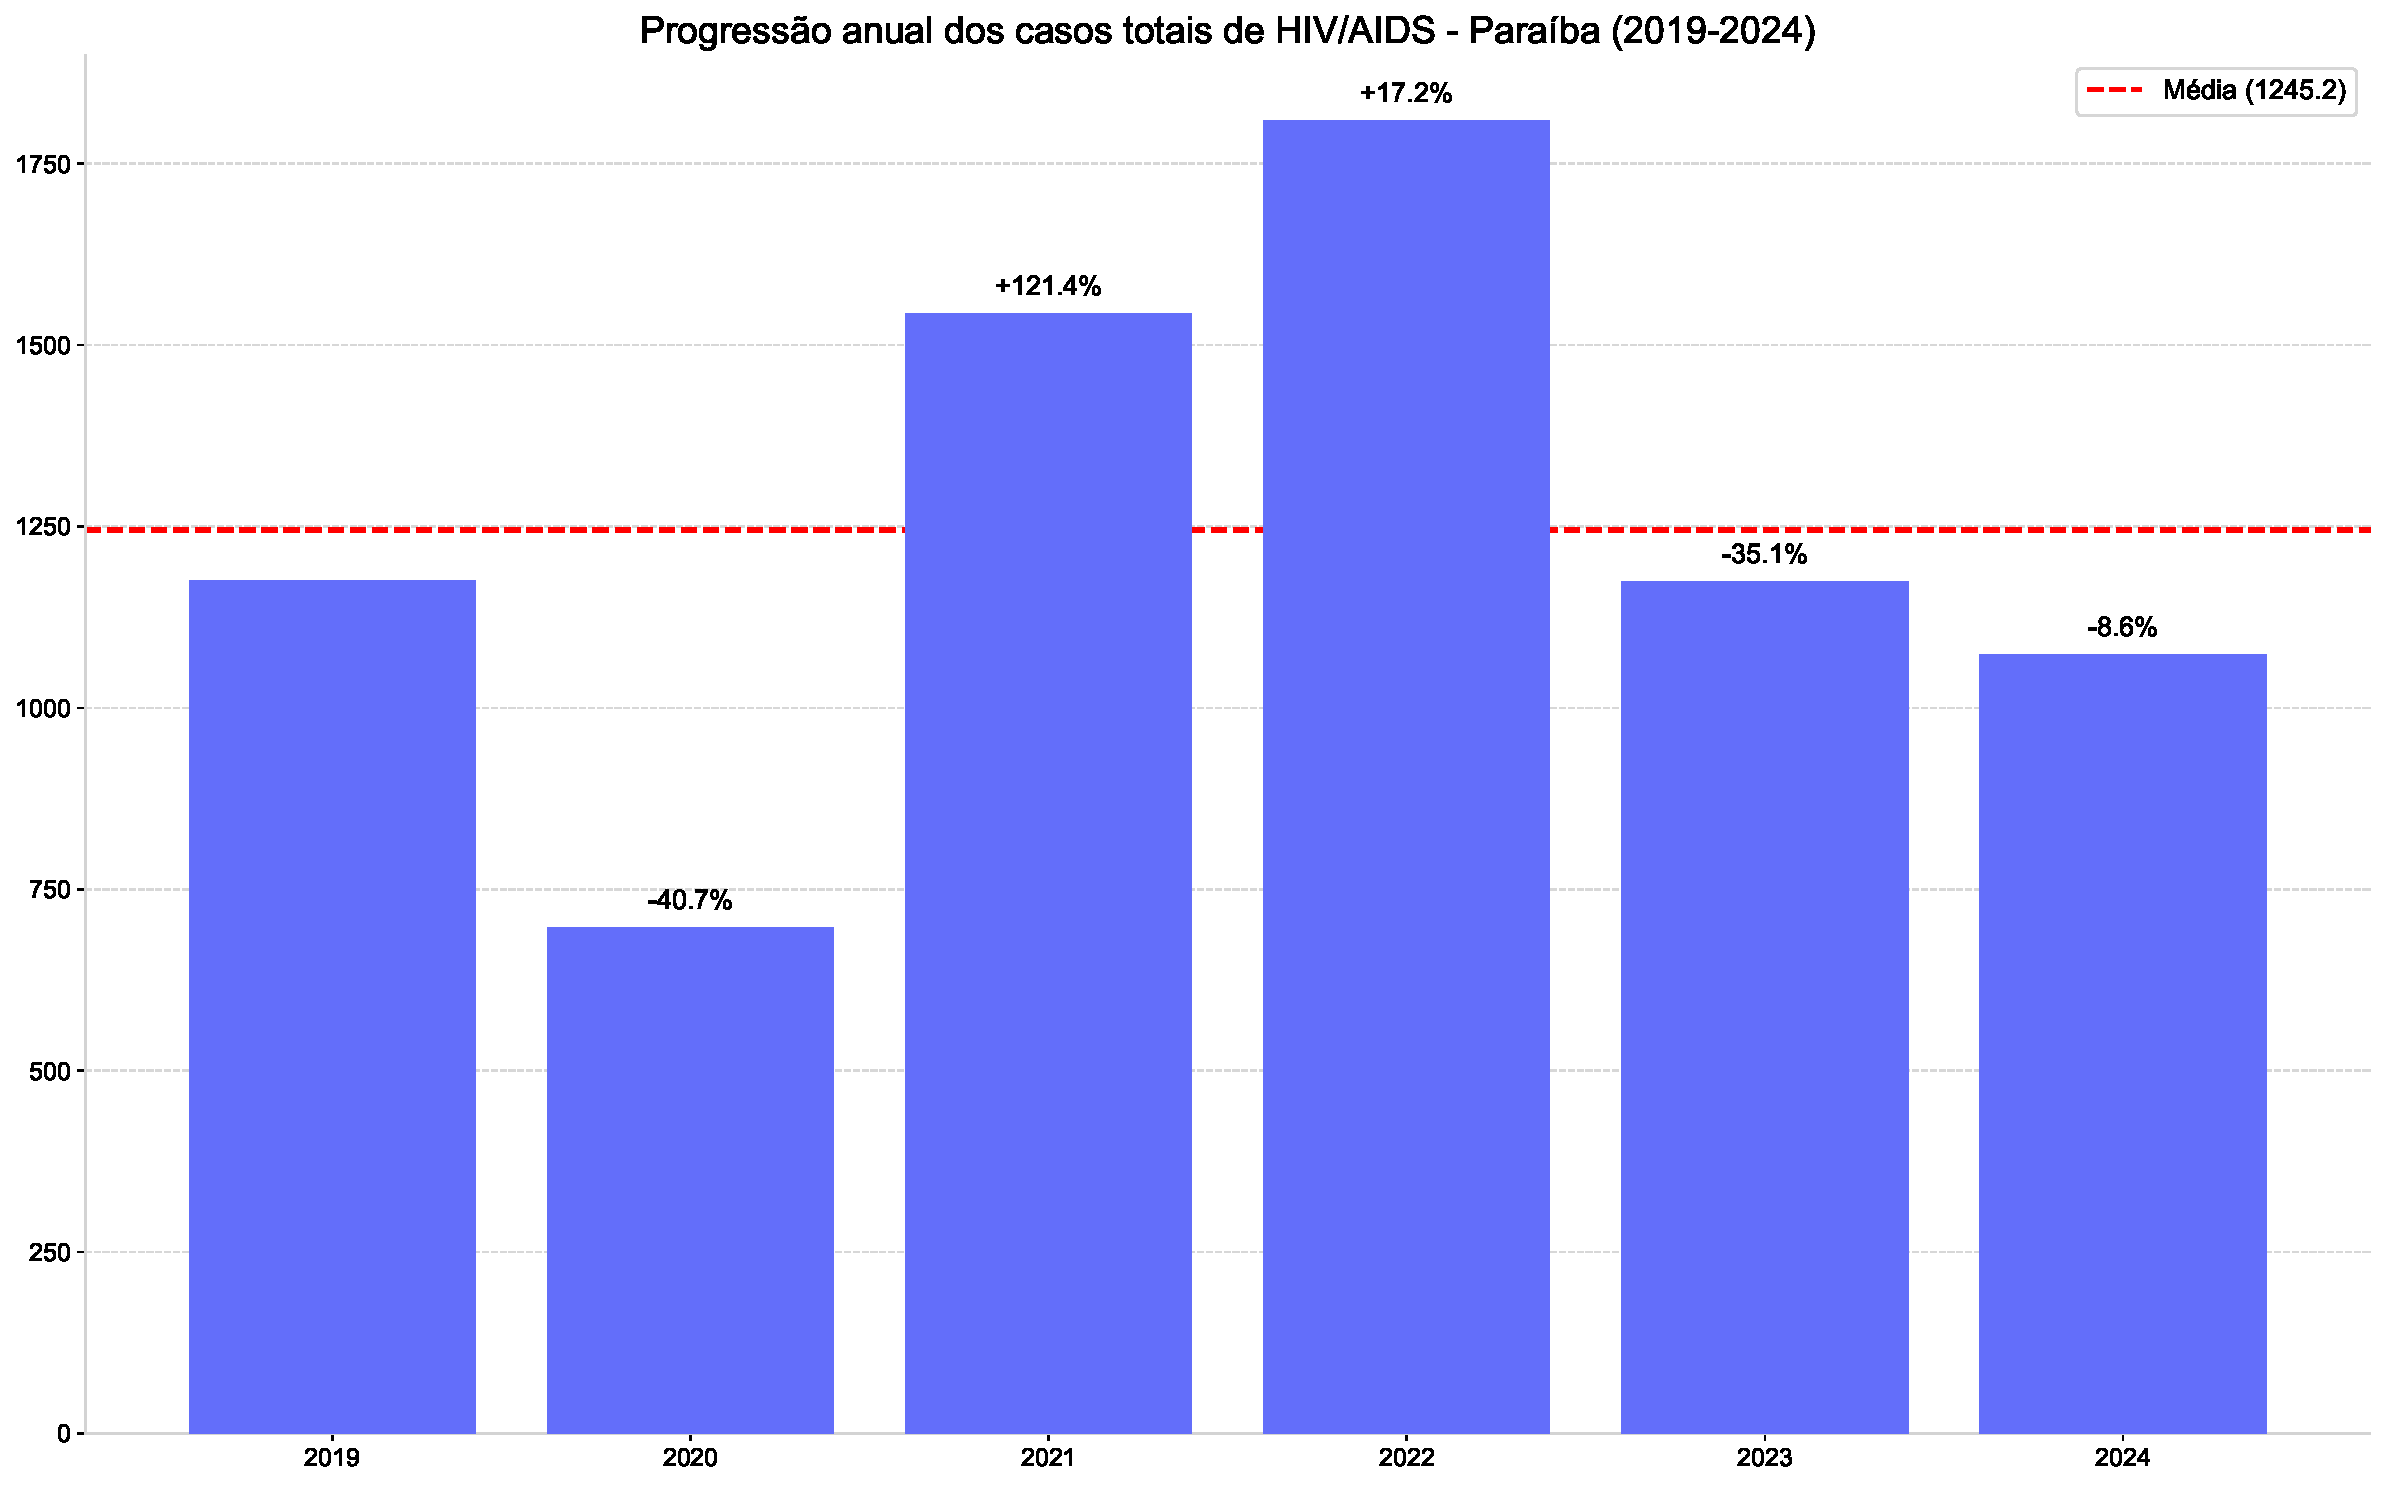
\includegraphics[width=\linewidth]{../figs/hiv_aids_pb_2019-2022.pdf}
    \caption{Evolução temporal dos casos de HIV/AIDS na Paraíba (2019-2024)}
    \label{fig:evolucao_temporal}
\end{figure}

\textbf{Distribuição por Sexo}

A Figura 3, por sua vez, indica a distribuição temporal estratificada por sexo. Em relação à visualização, adotou-se o gráfico de linhas com diferenciação cromática: azul para o sexo masculino e rosa para o feminino, seguindo convenções visuais estabelecidas.

\begin{figure}[H]
    \centering
    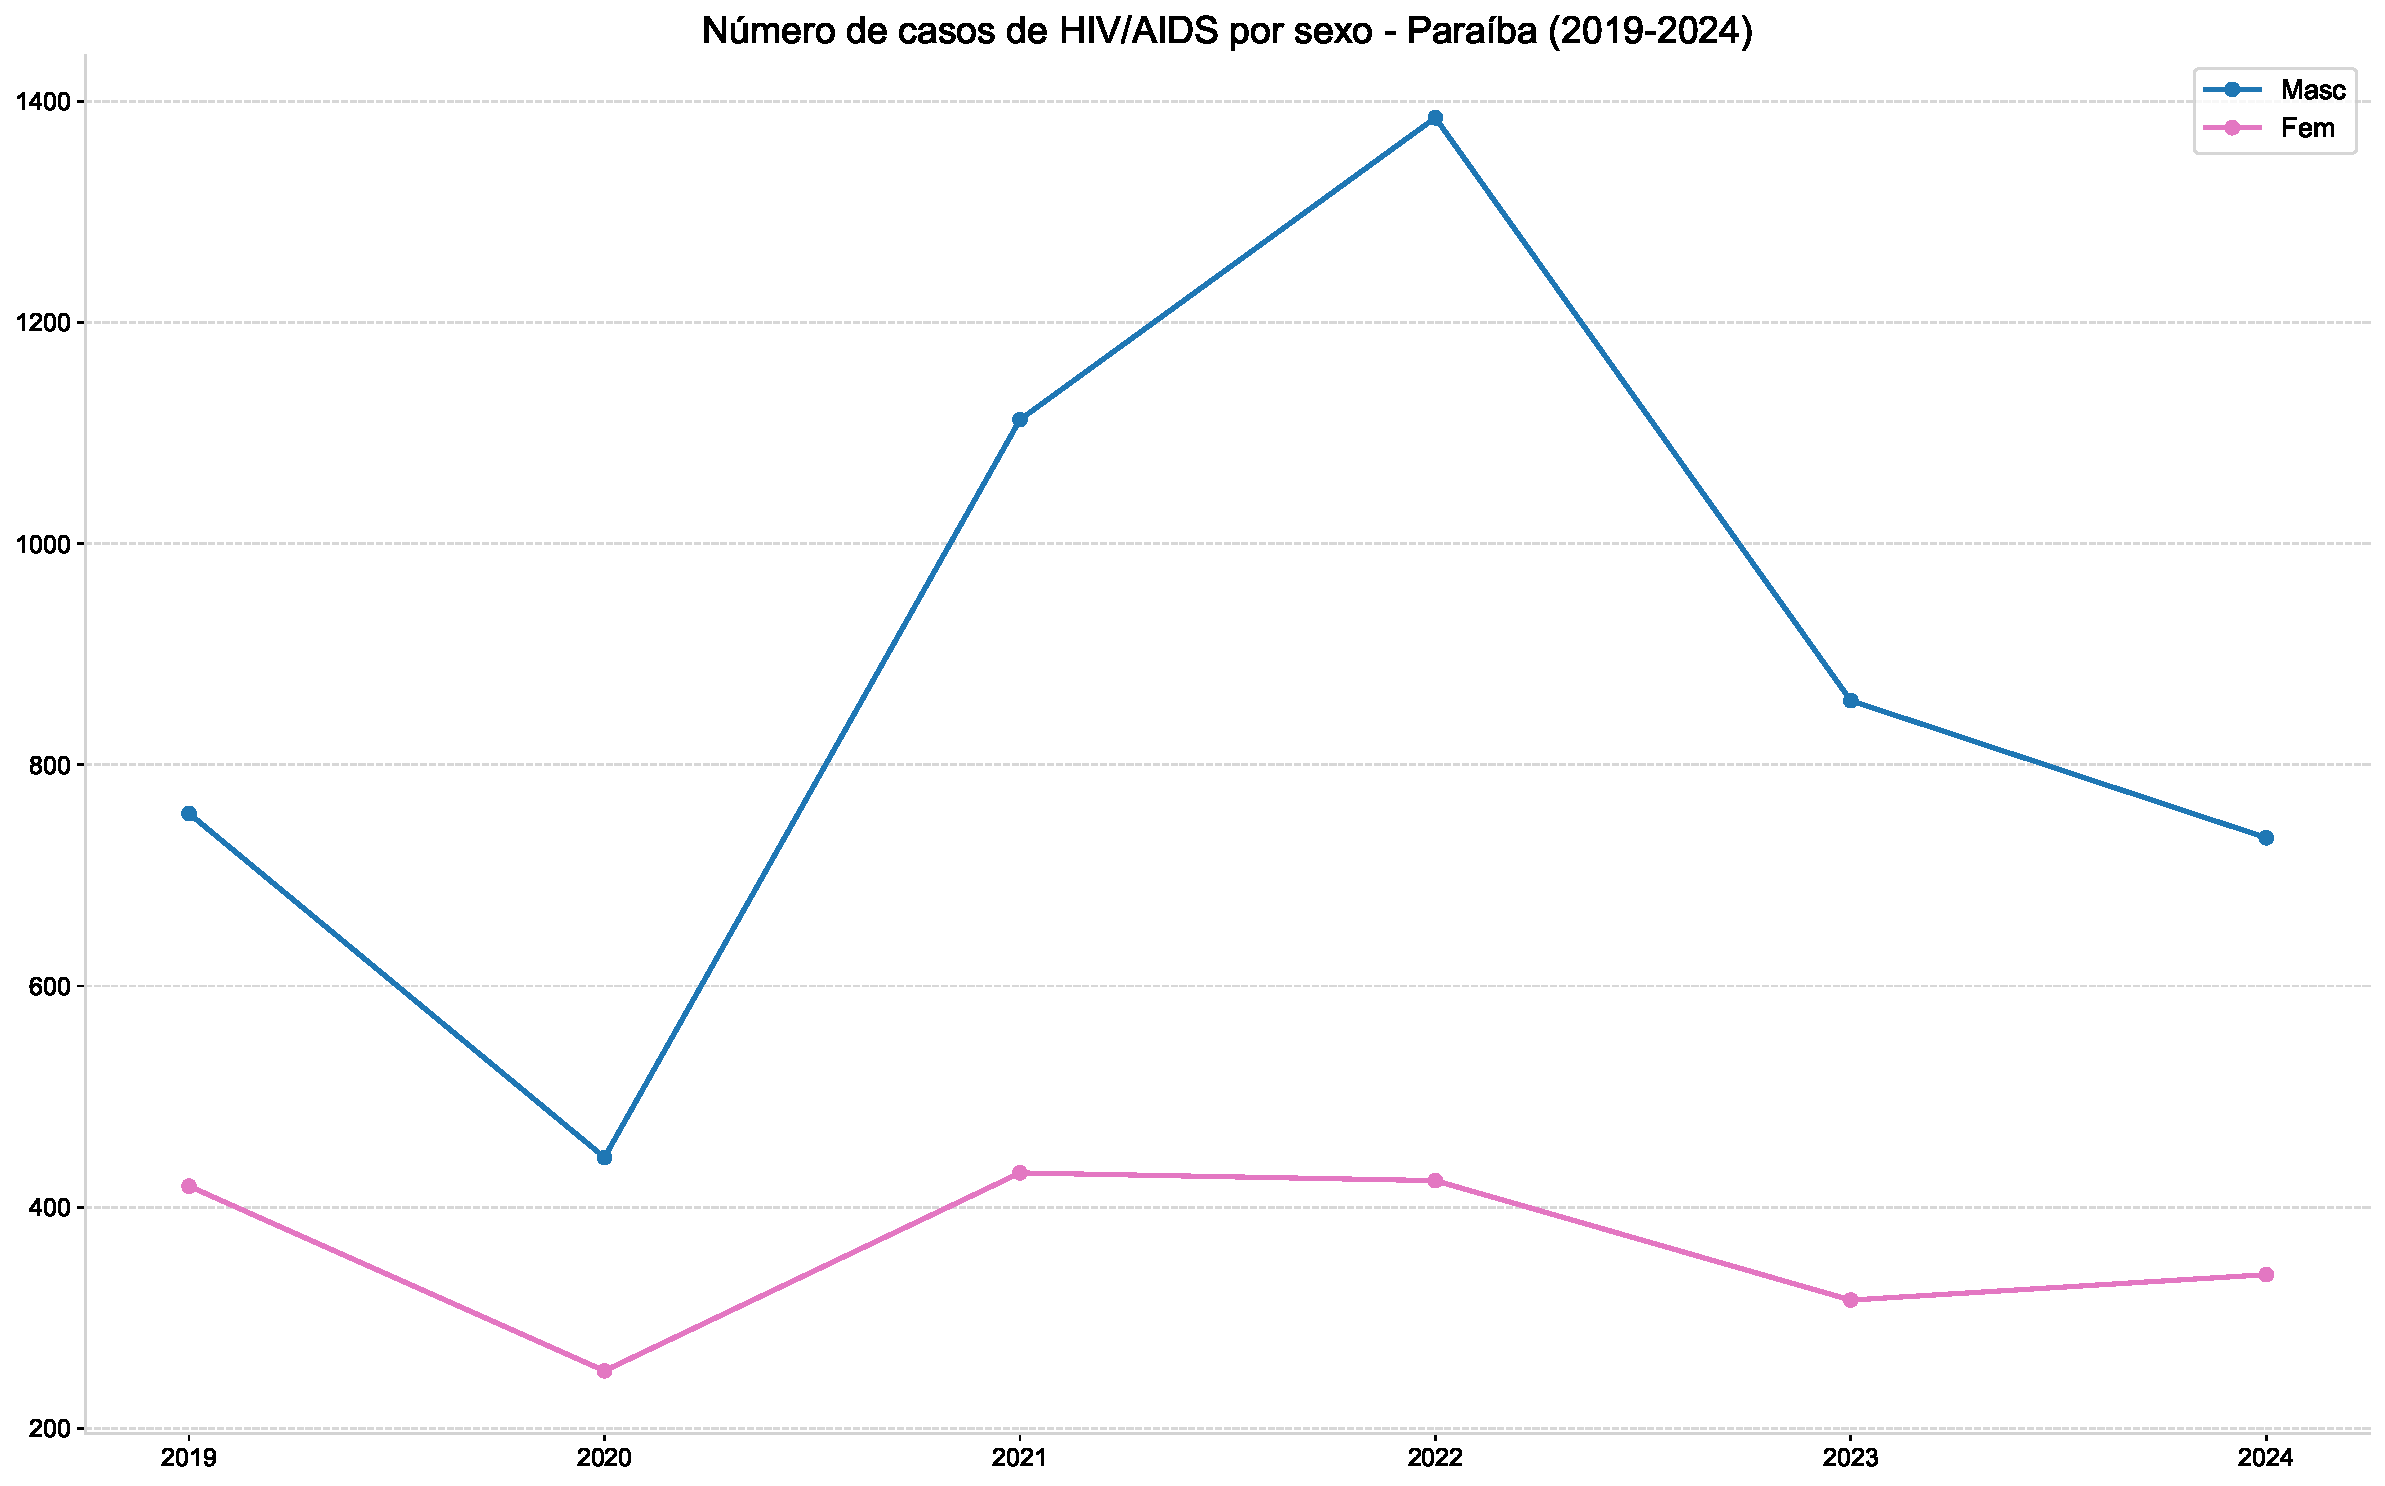
\includegraphics[width=\linewidth]{../figs/hiv_aids_pb_sex_2019-2022.pdf}
    \caption{Distribuição de casos de HIV/AIDS por sexo na Paraíba (2019-2024)}
    \label{fig:distribuicao_sexo}
\end{figure}

\textbf{Casos por Faixa Etária e Sexo}

A Figura 4 aponta a distribuição dos casos segundo faixa etária estratificada por sexo. Nesta visualização, foi adotada uma composição de barras agrupadas com diferenciação cromática entre os sexos: azul para masculino e laranja para feminino. Pode-se notar também a presença de dois subgráficos lado a lado, sendo o primeiro com barras em tons de cinza para visualização geral e o segundo com as barras agrupadas coloridas, facilitando a comparação entre os sexos dentro de cada faixa etária.

\begin{figure}[H]
    \centering
    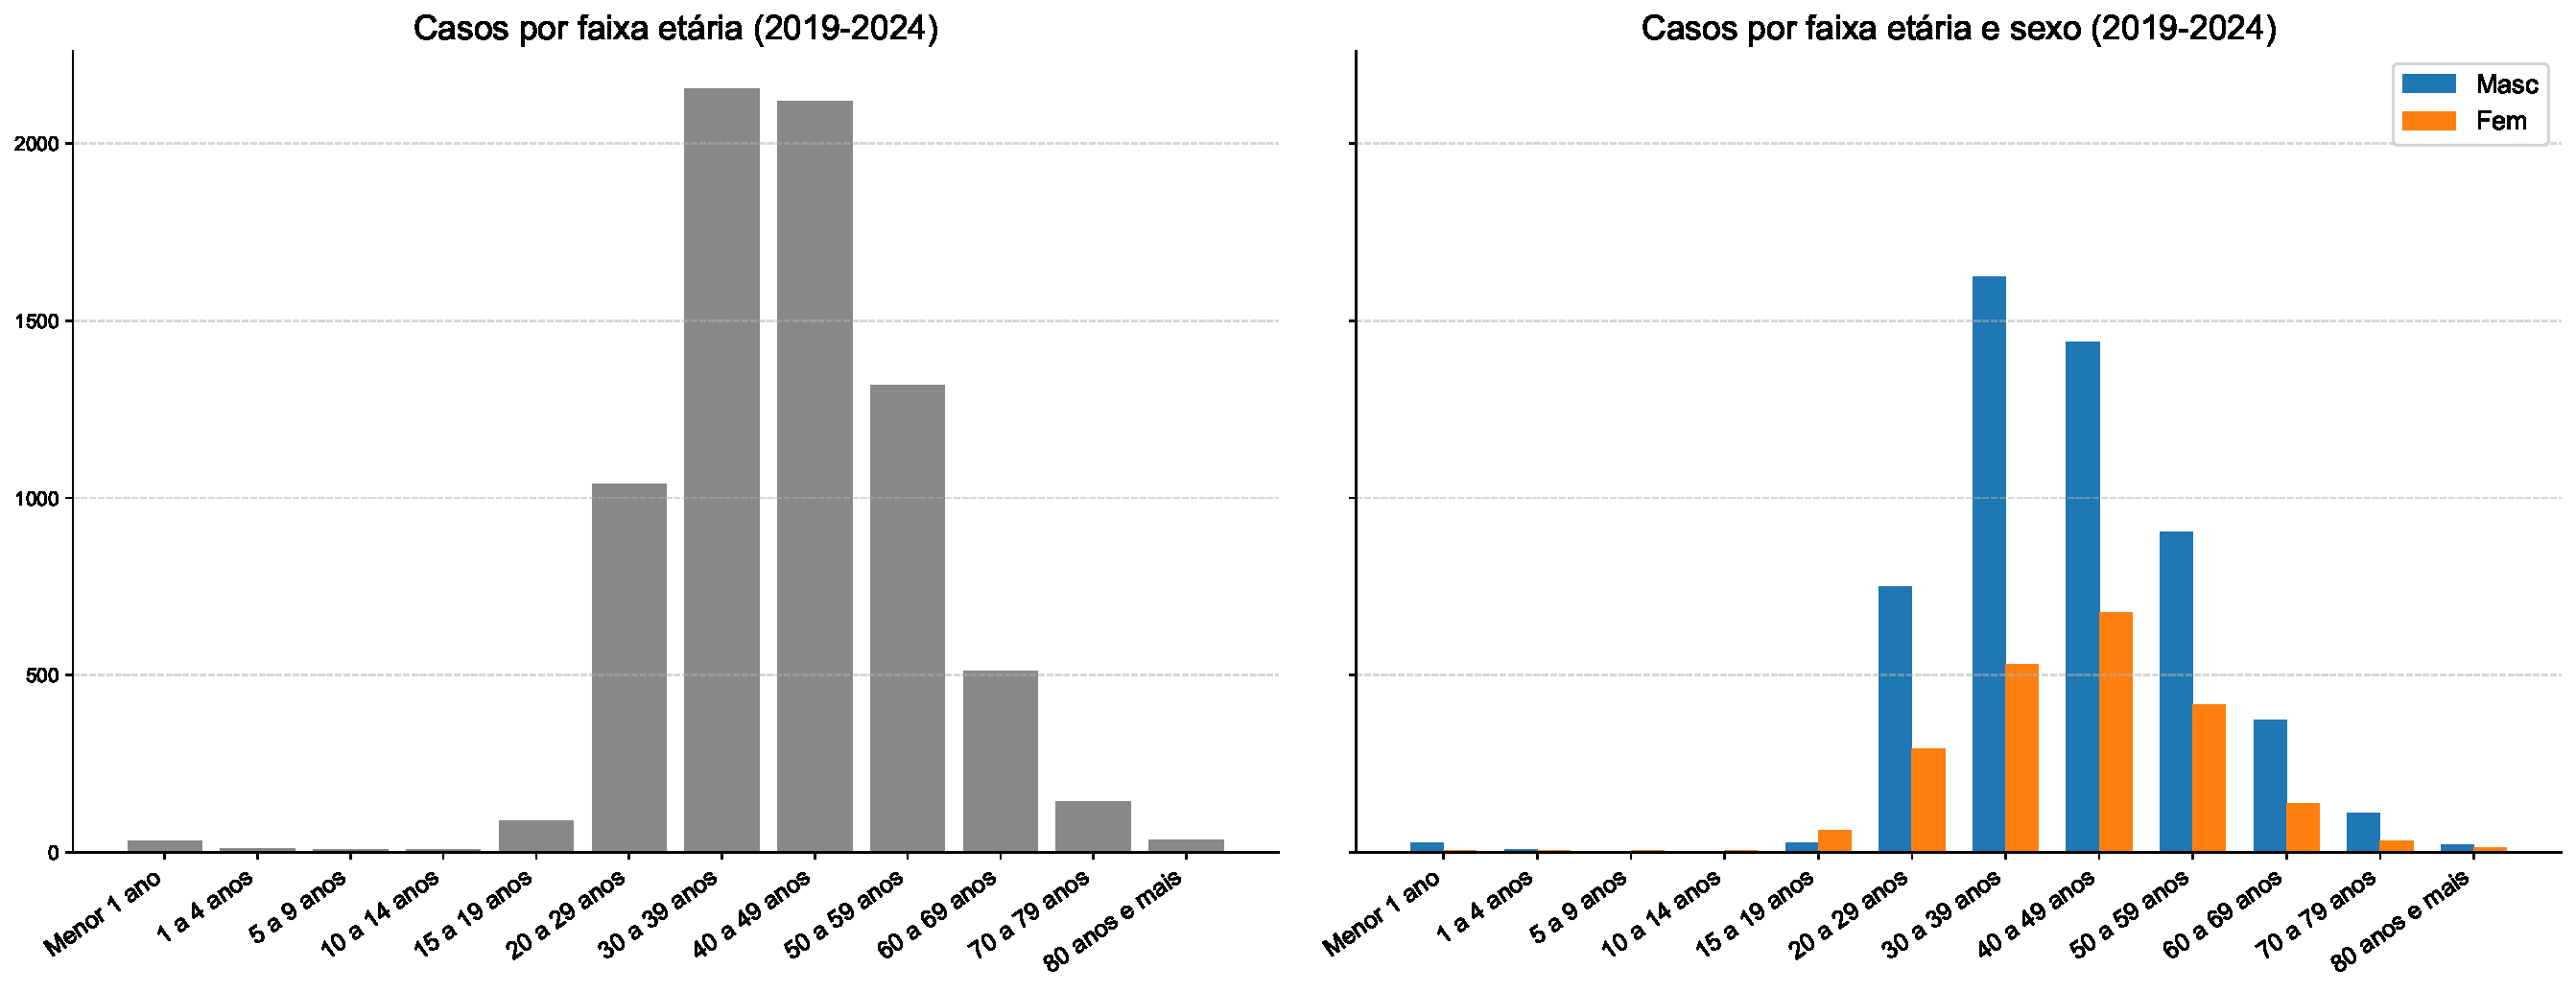
\includegraphics[width=\linewidth]{../figs/hiv_aids_pb_sex_age_2019-2022.pdf}
    \caption{Casos de HIV/AIDS por faixa etária e sexo na Paraíba (2019-2024)}
    \label{fig:faixa_etaria_sexo}
\end{figure}

\textbf{Distribuição Geográfica Municipal}

A Figura 5, por sua vez, representa a distribuição espacial através de mapa coroplético. Do ponto de vista visual, adotou-se uma escala de cores em gradiente viridis, onde tonalidades mais escuras indicam maiores concentrações de casos por 100.000 habitantes. Observa-se também a presença de uma barra de legenda lateral, facilitando a interpretação quantitativa das cores, e contornos municipais bem definidos em preto, conferindo clareza na delimitação territorial.

\begin{figure}[H]
    \centering
    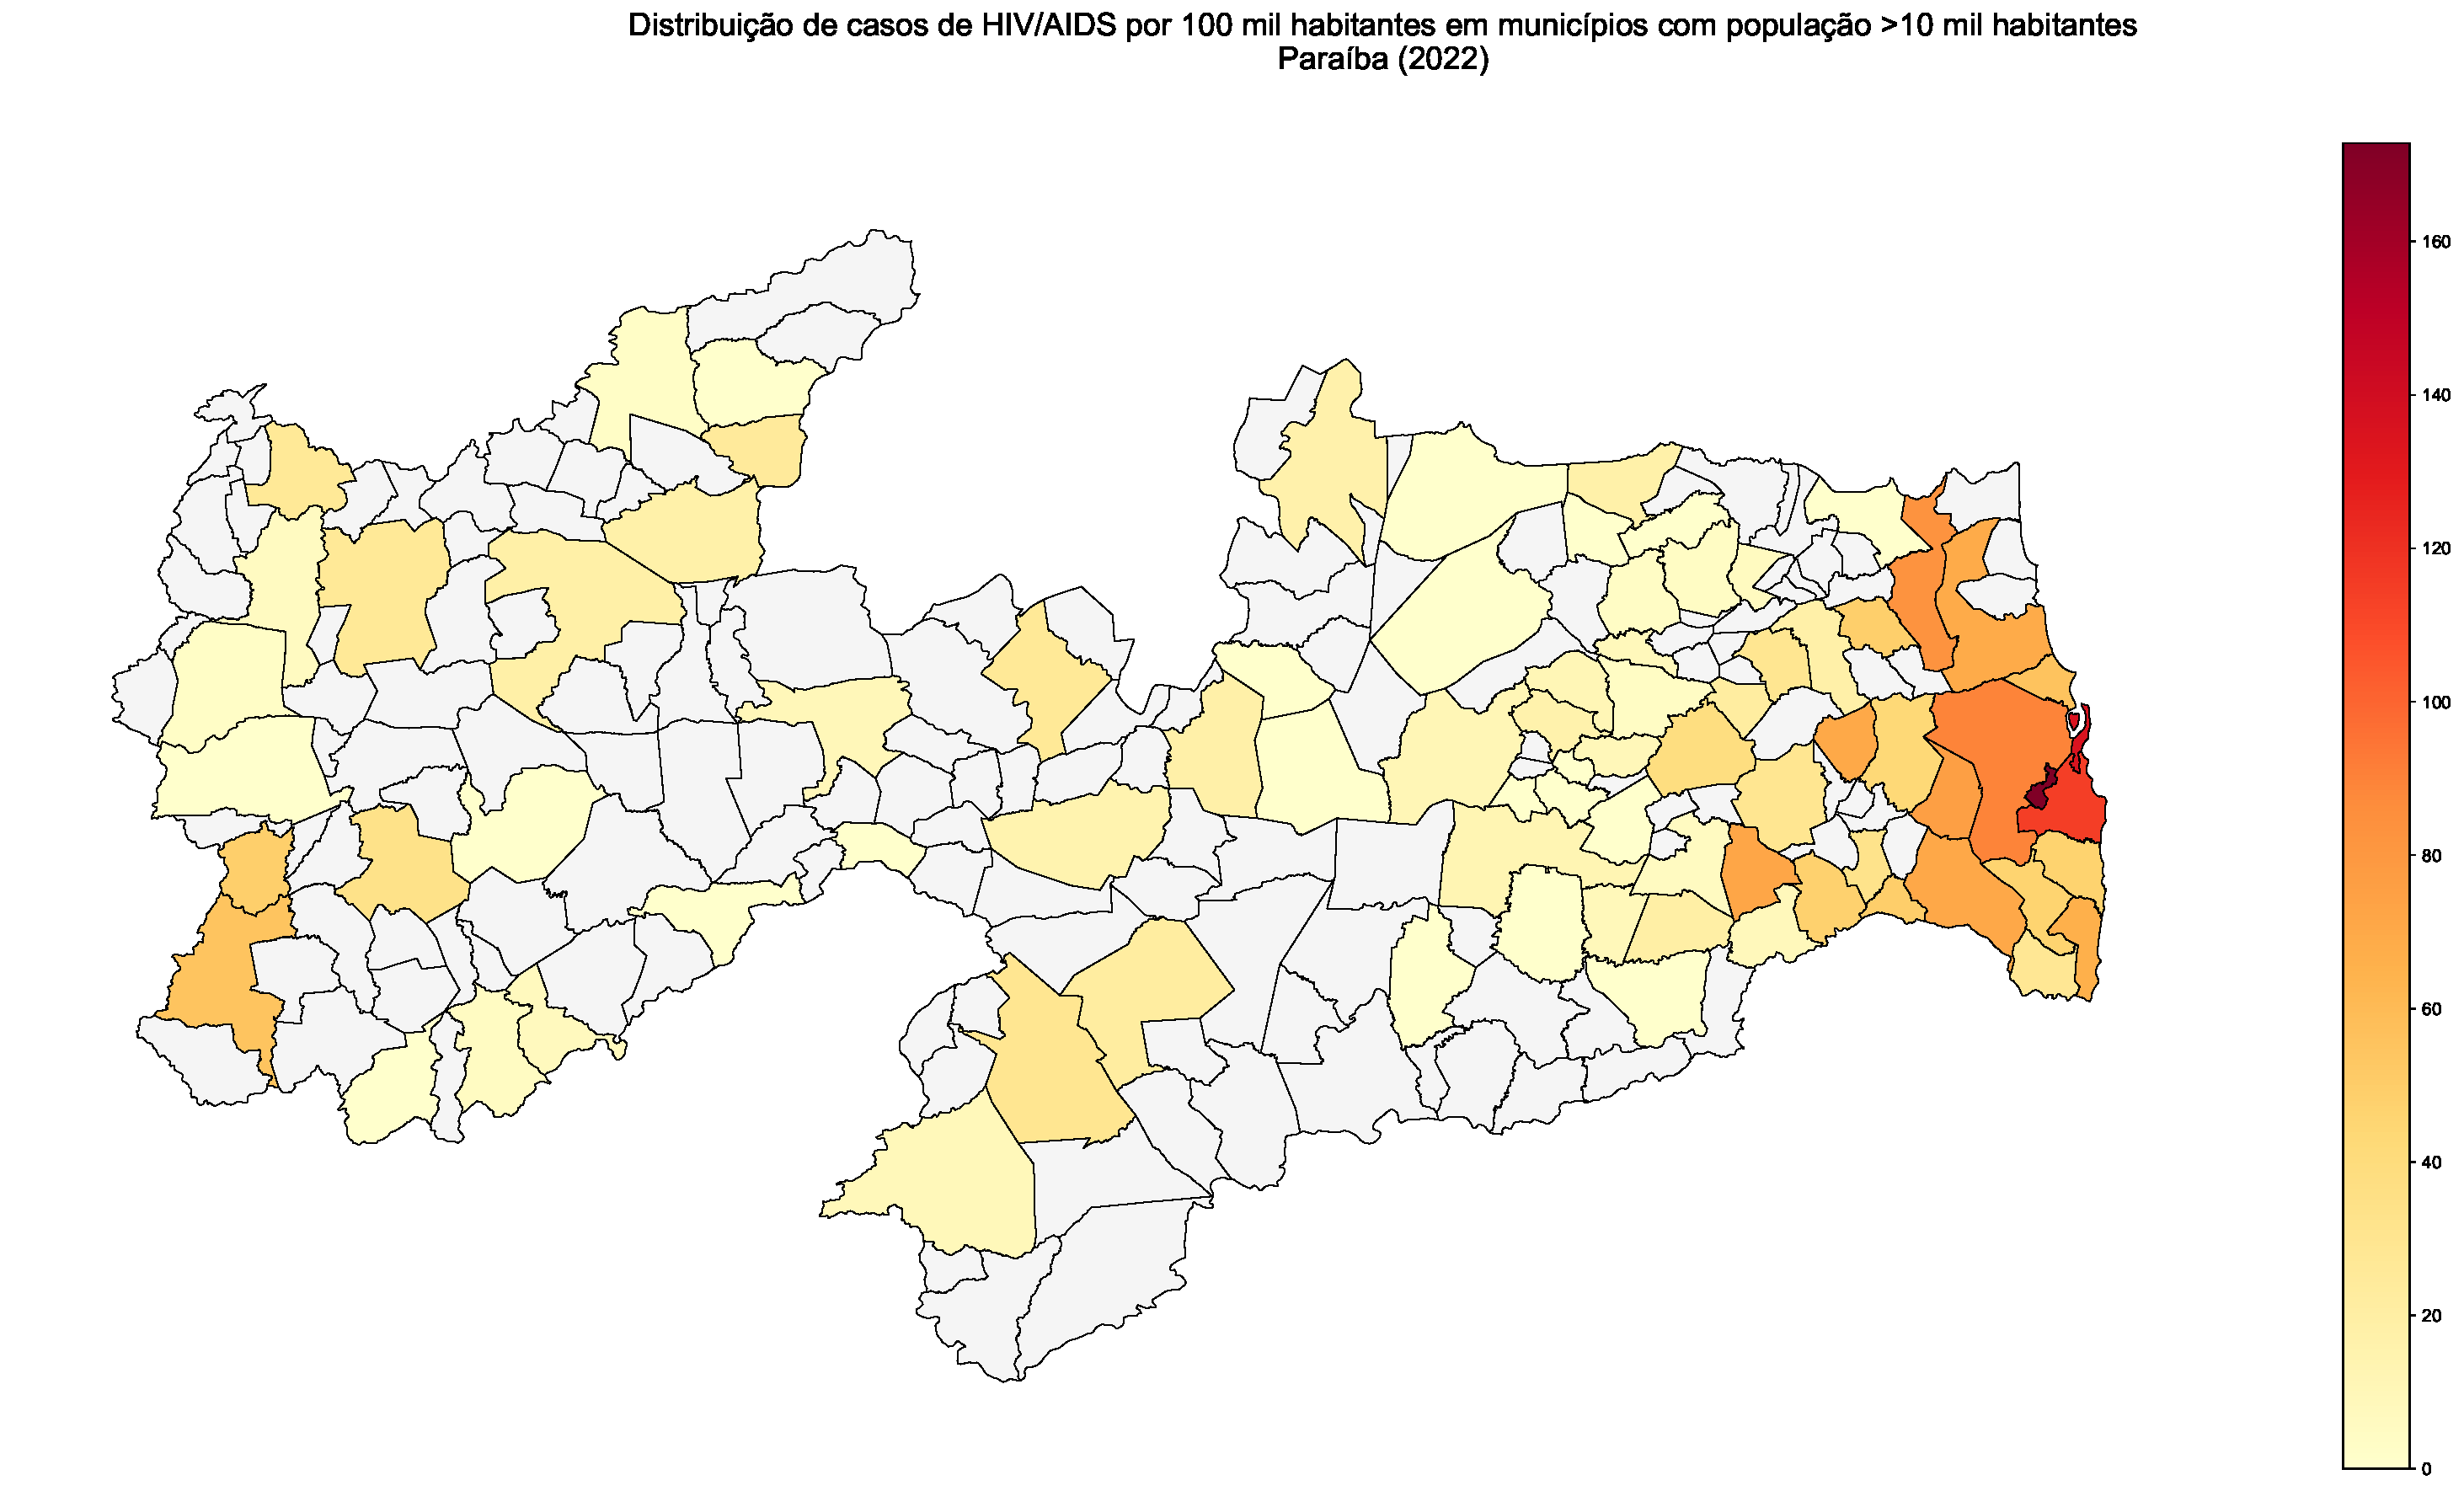
\includegraphics[width=\linewidth]{../figs/hiv_aids_pb_municipios_2022.pdf}
    \caption{Distribuição geográfica de casos (2022)}
    \label{fig:mapa_municipios}
\end{figure}

\textbf{Ranking Municipal por Taxas}

Por fim, a Figura 6 apresenta o ranking dos municípios com maiores taxas de incidência. Em relação à visualização, utilizou-se um gráfico de barras horizontais em gradiente de cores, variando de tons mais escuros (azul-violeta) para mais claros (verde-amarelo) conforme a magnitude das taxas. Pode-se verificar também a presença de rótulos municipais rotacionados, mecanismo que facilita a leitura e identificação dos municípios prioritários.

\begin{figure}[H]
    \centering
    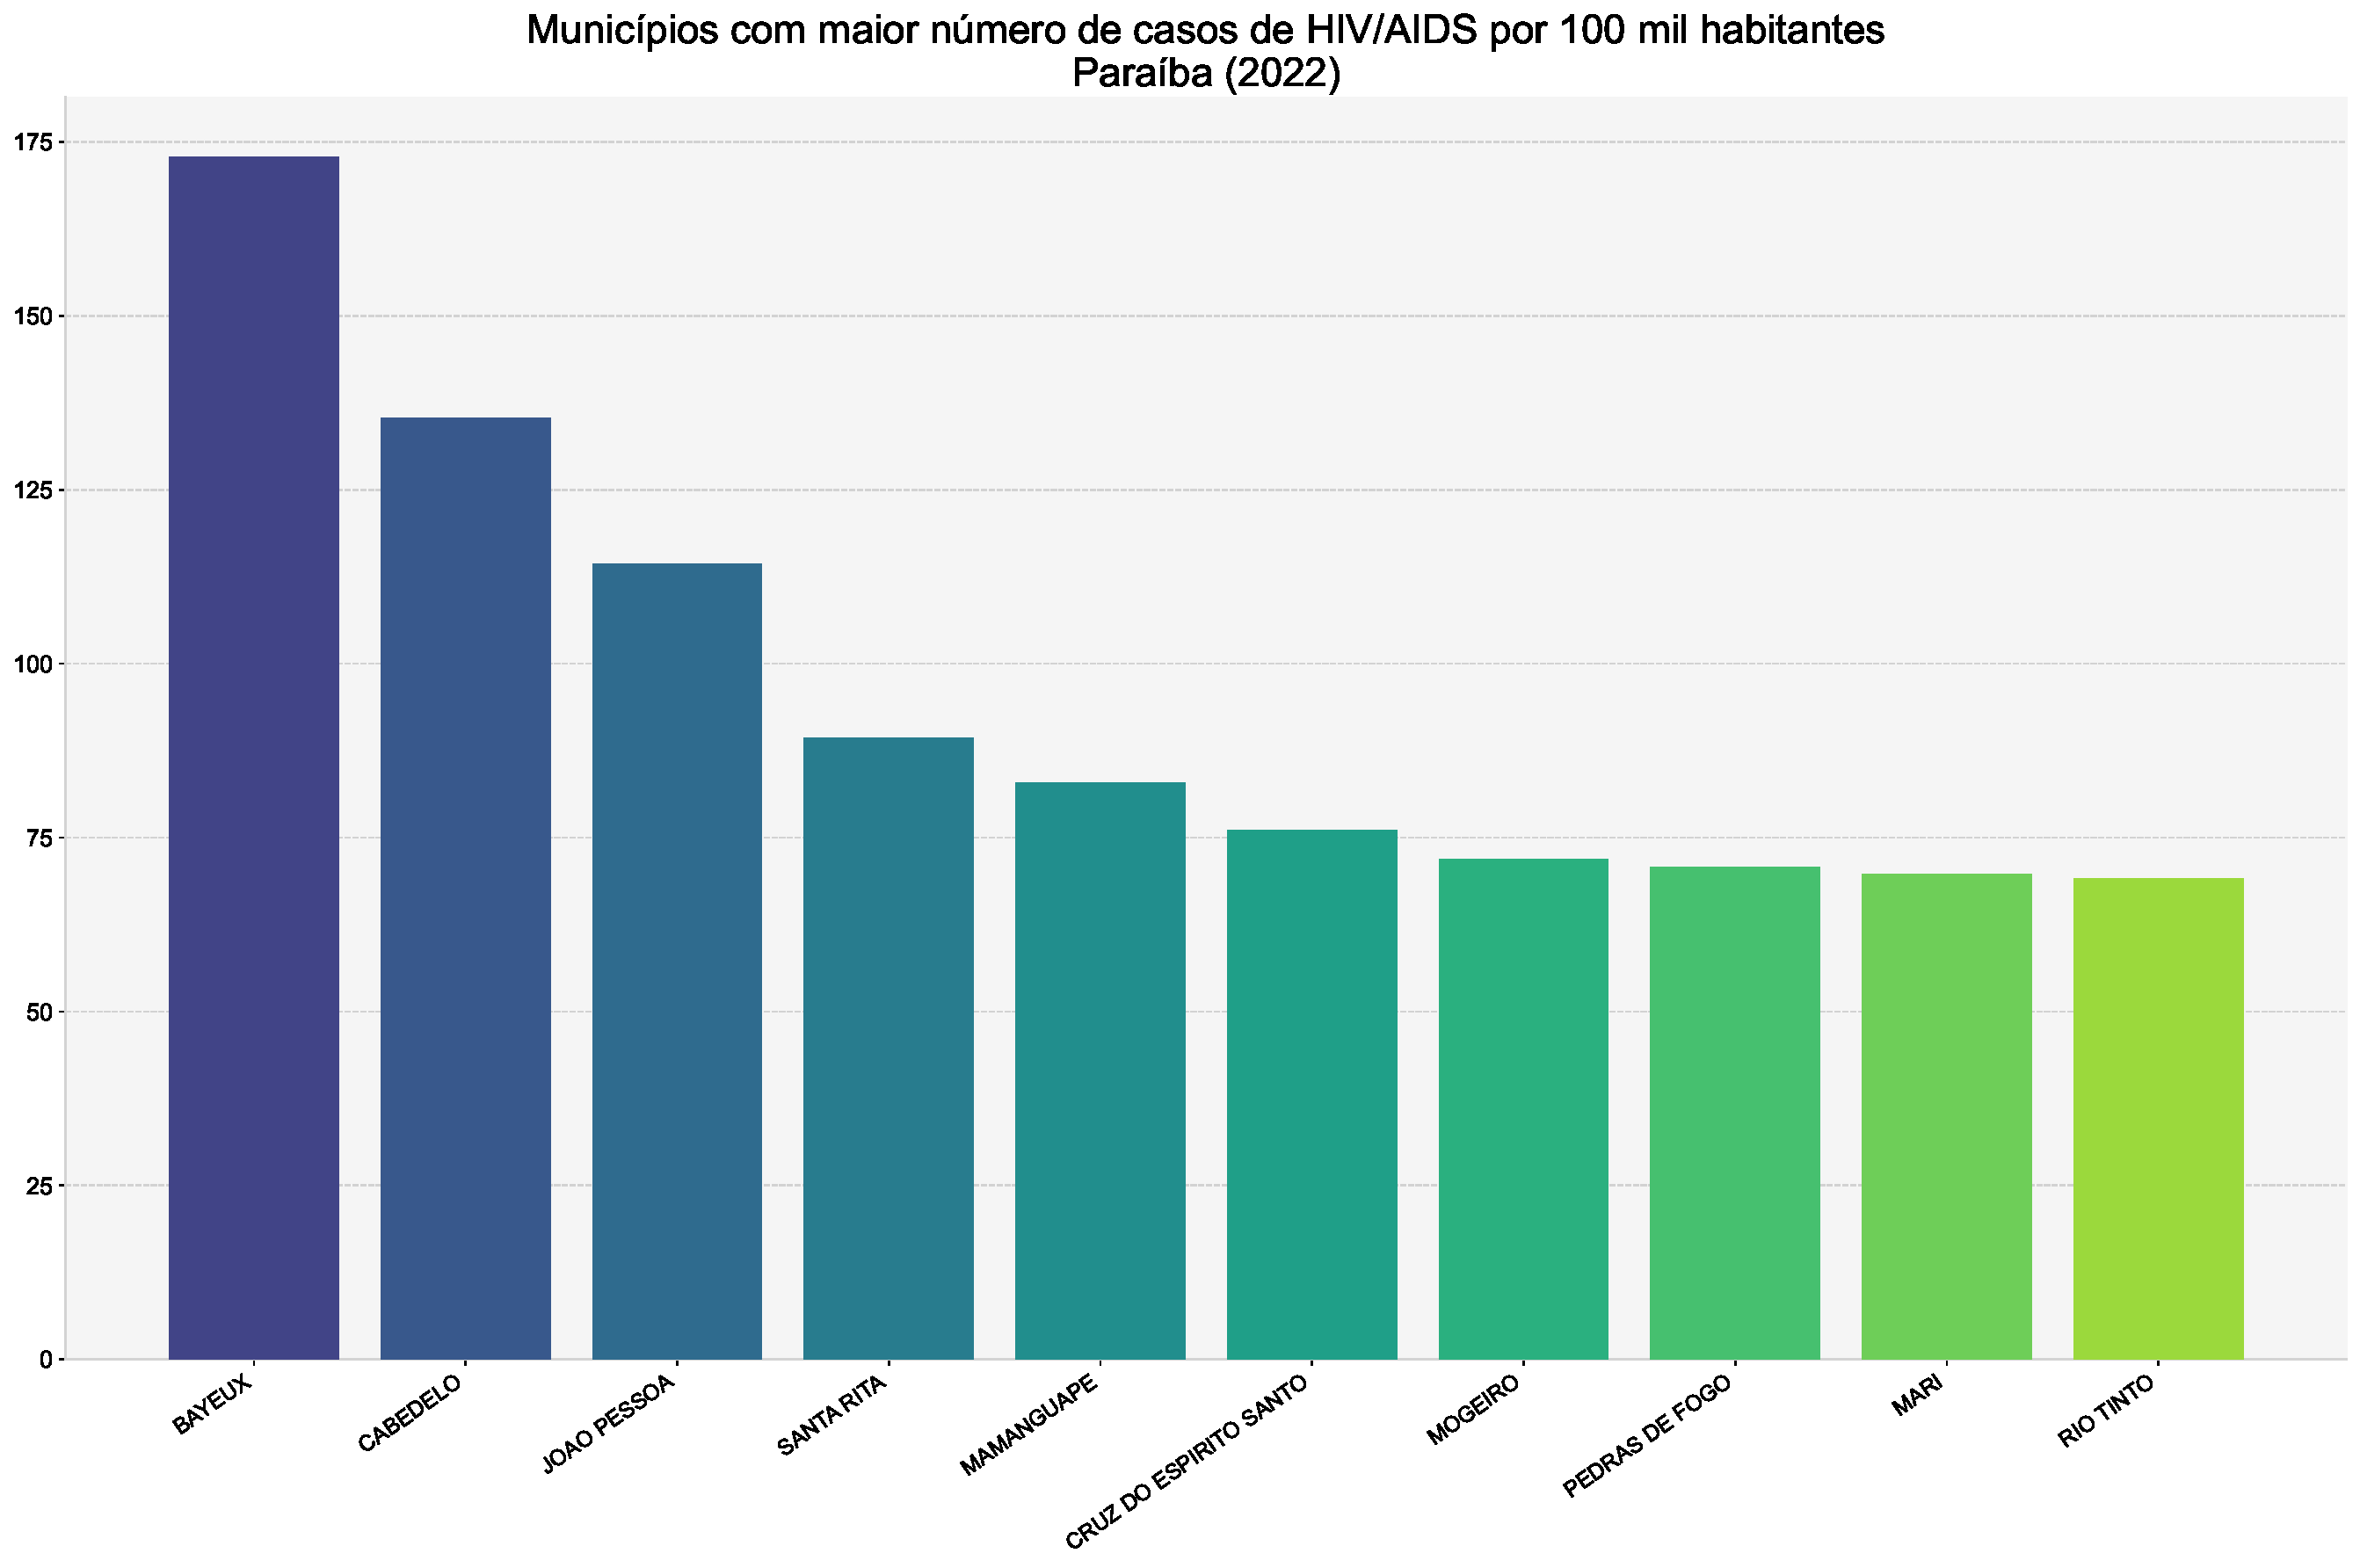
\includegraphics[width=\linewidth]{../figs/hiv_aids_pb_top_mun_2022.pdf}
    \caption{Municípios da Paraíba com maiores taxas de HIV/AIDS por 100.000 habitantes (2022)}
    \label{fig:top_municipios}
\end{figure}

\section{Análise de dados}

A partir das representações visuais desenvolvidas, observa-se que o perfil epidemiológico do HIV/AIDS na Paraíba apresenta características bem definidas. O grupo mais vulnerável concentra-se na população masculina entre 30-49 anos, representando aproximadamente 40\% dos 7.471 casos registrados no período 2019-2024. A distribuição geográfica dos 1.809 casos de 2022 revela concentração na região metropolitana de João Pessoa, com Bayeux apresentando a maior taxa (172,8 casos/100.000 hab.), seguida pelos municípios litorâneos de Cabedelo e Santa Rita. 

A análise temporal evidencia impacto significativo da pandemia de COVID-19, com redução de 40,7\% dos casos em 2020, seguida de recuperação expressiva em 2021-2022. A estratificação por sexo mantém padrão consistente de predominância masculina (razão 2,5:1), enquanto a distribuição etária confirma que adultos jovens constituem o grupo de maior risco, demandando estratégias preventivas direcionadas.

\section{Takeaways}

\textbf{1. Perfil de Risco Definido:} Homens de 30-49 anos representam o grupo mais vulnerável ao HIV/AIDS na Paraíba, concentrando a maioria dos casos e demandando campanhas preventivas específicas para este segmento populacional.

\textbf{2. Concentração Geográfica Estratégica:} A região metropolitana de João Pessoa, especialmente os municípios de Bayeux, Cabedelo e Santa Rita, apresenta as maiores taxas de incidência, indicando a necessidade de intensificação dos serviços de testagem e prevenção nestas localidades.

\textbf{3. Impacto de Fatores Externos:} A pandemia de COVID-19 alterou significativamente os padrões de diagnóstico, evidenciando a importância de sistemas de vigilância epidemiológica robustos e resilientes para garantir continuidade do monitoramento e controle da doença.

\end{multicols}

% Bibliografia
\section{Referências}
\printbibliography[heading=none]

\end{document}